\documentclass{article}
\usepackage[utf8]{inputenc}
\usepackage{xcolor}
%\usepackage[a4paper]{geometry}%
\usepackage{tikz}
\usetikzlibrary{shapes.geometric, arrows, decorations.pathreplacing, positioning}

\title{What the Frick}
\author{David Kasofsky}
%macros%
\newcommand{\defchar}[2]{%
  \expandafter\newcommand\csname c#1\endcsname{\textcolor{green}{\textbf{#2}}}%
}
\newcommand{\defroom}[2]{%
  \expandafter\newcommand\csname r#1\endcsname{\textcolor{red}{\textbf{#2}}}%
}
\newcommand{\defitem}[2]{%
  \expandafter\newcommand\csname i#1\endcsname{\textcolor{blue}{\textbf{#2}}}%
}
\newcommand{\defpainting}[2]{%
  \expandafter\newcommand\csname p#1\endcsname{\textcolor{violet}{\textbf{#2}}}%
}

%chart shapes%
\tikzstyle{plain} = [rectangle, rounded corners, minimum width=3cm, minimum height=0.66cm, text centered, draw=black]%
%\tikzstyle{plain} = [rectangle]
\tikzstyle{arrow} = [thick,->,>=stealth]

%rooms%
\defroom{entrance}{Museum Entrance}
\defroom{entry}{Entry Hall}
\defroom{reception}{Reception Hall}
\defroom{anter}{Ante Room}
\defroom{boucher}{Boucher Room}
\defroom{dining}{Dining Room}
\defroom{evest}{East Vestibule}
\defroom{wvest}{West Vestibule}
\defroom{living}{Living Hall}
\defroom{library}{Library}
\defroom{music}{Music Room}
\defroom{wgall}{West Gallery}
\defroom{egall}{East Gallery}
\defroom{enamels}{Enamels Room}
\defroom{oval}{Oval Room}
\defroom{5thgarden}{5th Avenue Garden}
\defroom{70thgarden}{70th Street Garden}
\defroom{gardencourt}{Garden Court}
\defroom{shall}{South Hall}
\defroom{nhall}{North Hall}
\defroom{portico}{Portico Gallery}
\defroom{cabinet}{Cabinet Gallery}
\defroom{llngall}{Lower Level North Gallery}
\defroom{llsgall}{Lower Level South Gallery}
\defroom{llvest}{Lower Level Vestibule}

%characters%
\defchar{yl}{Young Lady}
\defchar{frick}{H.C. Frick}
\defchar{curator}{The Curator}
\defchar{guide}{Audio Guide}
\defchar{bagchecker}{Bag Check Person}
\defchar{usher}{Usher}
\defchar{admissions}{Admission Person}
\defchar{helpdesk}{Help Desk Person}
\defchar{coughy}{Coughy}

%items%
\defitem{frickestateletter}{Letter from Frick Estate}
\defitem{ylbag}{Young Lady's Bag}
\defitem{bagcheckstub}{Bag Check Stub}
\defitem{ylcoat}{Young Lady's Coat}
\defitem{coatcheckstub}{Coat Check Stub}
\defitem{audioguide}{Audio Guide}
\defitem{frickskull}{Frick's Skull}
\defitem{feather}{Feather}

%paintings%
\defpainting{memlingman}{Portrait of a Man}
\defpainting{dally}{Grace Dalrymple Elliot}
\defpainting{rpjodrell}{Richard Paul Jodrell}
\defpainting{rembrandt}{Rembrandt van Rijn}%, please call me Harmenszoon
\defpainting{skipworth}{Lady Skipworth}
\defpainting{etaylor}{Lady Taylor}
\defpainting{louisbust}{Louis XVI}

\begin{document}
%\tableofcontents{}%
\maketitle{}

\section*{Characters}
In order of importance:
\begin{description}
  \item[\cyl{}] - Protagonist. Art History student; last living Frick relative.
  \item[\cfrick{}] - Primary antagonist. 19th Century Industrialist and Voodoo Lich. Soul trapped in the Art World. His portrait is a horcrux. 
  \item[\ccurator{}] - Secondary antagonist. Museum Curator and Custodian of the Frick Estate. Bound to \cfrick{} by evil magic and serves as his henchman. Largo LeGrande-like character.
  \item[\iaudioguide{}] - Another \cfrick{} henchman. Leads \cyl{} into \cfrick{}'s traps. It is secretly a Voodoo priest and performs evil rituals for \cfrick{}. 
  \item[\ccoughy{}] - A nice usher who helps \cyl{} but doesn't speak much English. African, 40-50 years old, bit portly, bald, and coughs periodically. He is later forced against his will to subdue \cyl{} after \iaudioguide{} possesses him.
\end{description}

\section*{Summary}
\cyl{} receives a letter from \ccurator{}. The letter says she is a long-lost relative of \cfrick{} and is invited to the Frick Museum Centennial. In fact \ccurator{} and \cfrick{} are trying to find a living Frick descendant for nefarious purposes. \cyl{} goes to the Centennial and meets \ccurator{}. In a roped-off part of the museum, \cyl{} discovers a magical portrait that can talk. At the portrait's bidding, she enters the Art World via another painting that acts as a portal. When she returns to the museum she finds the party is over and she is locked inside the museum. \cyl{} resolves to investigate the magic paintings in the meantime. \cyl{} ultimately discovers that \cfrick{} seeks to use her body as a vessel so his soul can return from the Art World to the Real World. \cyl{} defeats \cfrick{} and banishes him to the Void - for now.

\subsection{Plot Chart}

\begin{center}
  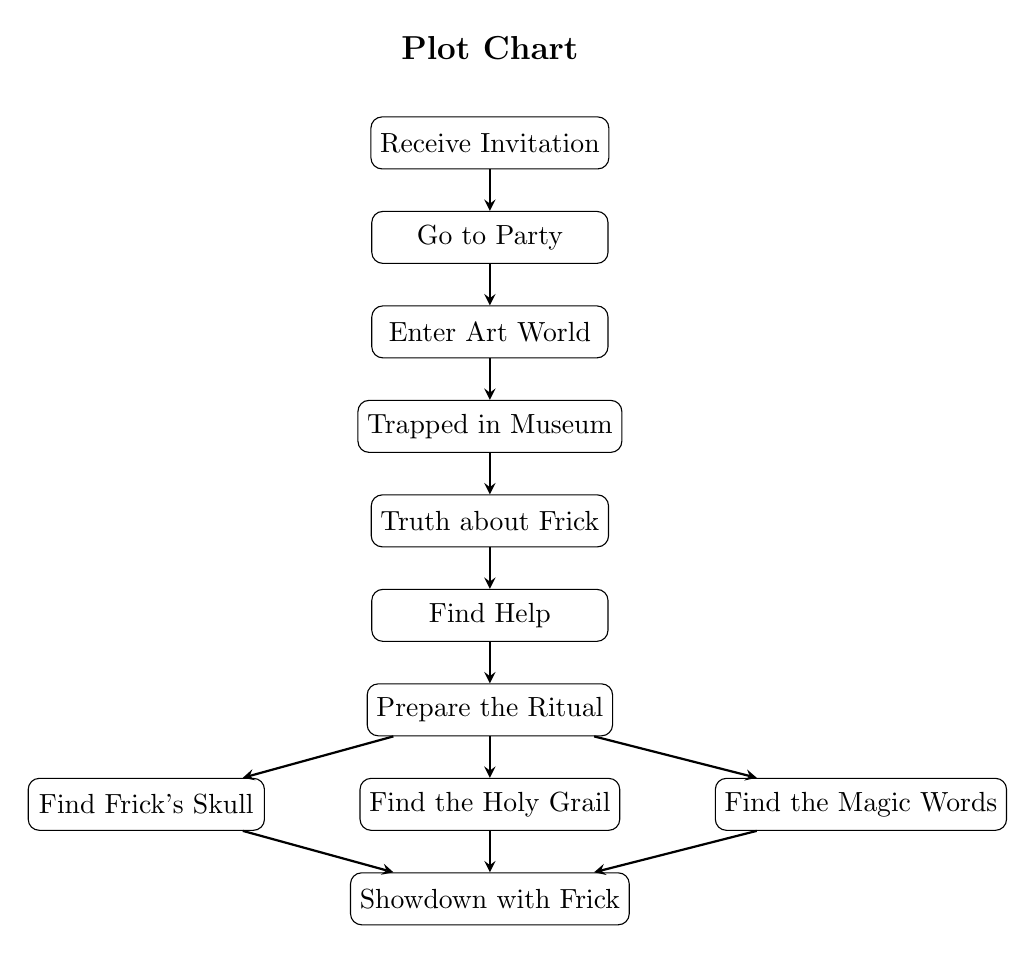
\begin{tikzpicture}[node distance=1.2cm]
  % nodes
    \node (invitation) [plain] {Receive Invitation};
    \node (party) [plain, below of = invitation] {Go to Party};
    \node (artworld) [plain, below of = party] {Enter Art World};
    \node (trapped) [plain, below of = artworld] {Trapped in Museum};
    \node (learntruth) [plain, below of = trapped] {Truth about Frick};
    \node (findhelp) [plain, below of = learntruth] {Find Help};
    \node (prepareritual) [plain, below of = findhelp] {Prepare the Ritual};
    \node (holygrail) [plain, below of = prepareritual] {Find the Holy Grail};
    \node (frickskull) [plain, left = of holygrail] {Find Frick's Skull};
    \node (incantation) [plain, right = of holygrail] {Find the Magic Words};
    \node (showdown) [plain, below of = holygrail] {Showdown with Frick};
    \node (pctitle) [font=\large\bfseries, above of = invitation] {Plot Chart};
  %arrows
    \draw [arrow] (invitation) -- (party);
    \draw [arrow] (party) -- (artworld);
    \draw [arrow] (artworld) -- (trapped);
    \draw [arrow] (trapped) -- (learntruth);
    \draw [arrow] (learntruth) -- (findhelp);
    \draw [arrow] (findhelp) -- (prepareritual);
    \draw [arrow] (prepareritual) -- (holygrail);
    \draw [arrow] (prepareritual) -- (frickskull);
    \draw [arrow] (prepareritual) -- (incantation);
    \draw [arrow] (holygrail) -- (showdown);
    \draw [arrow] (frickskull) -- (showdown);
    \draw [arrow] (incantation) -- (showdown);
  \end{tikzpicture}
\end{center}

\cyl{} receives a mysterious letter in the mail containing an invitation to The Frick Collection Bicentennial Event. \cyl{} attends and finds it to be a stuffy party full of old effete rich people confined to a corner of the museum. Bored, \cyl{} sneaks out of the party to explore the museum. \cyl{} is accidentally transported to the magical Art World, and when she returns to the Museum she finds that it is frozen in time. \cyl{} learns that Frick is behind the magic and that she must complete the spell to confront Frick and escape.

\section{Receive Invitation}
Opening cutscene. \cyl{} receives a letter in the mail. Inside is an invitation to the Frick Bicentennial Party, hosted at The Frick Collection. As an Art History student, \cyl{} is intrigued.

\section{Go to Party}
\cyl{} arrives at the museum. She is greeted in the \rentry{} by an usher and directed to the party. There is an usher standing near the entrance to the \rgardencourt{} and \rreception{} is roped off. The party is taking place in \revest{}, \rwvest{}, \rdining{}, \ranter{}, and \rboucher{}.




\newpage
\section{Chapter 1: Welcome to the Frick}
\begin{enumerate}
  \item initial inventory: \ifrickestateletter{}, \iylbag{}
  \item arrive at the \rentrance{}
  \item talk to \ccurator{} about family history 
  \item receive \iaudioguide
  \item explore museum while waiting for \ccurator{}
    \begin{itemize}
      \item perhaps \cyl{} is given suggestions for paintings to seek out (one in each room?)
      \item \pdally{}, \pmemlingman{}
    \end{itemize}
  \item trigger first magical painting encounter
    \begin{itemize}
      \item 
    \end{itemize}
\end{enumerate}
\subsection{Receive Letter}
The chapter opens with a cutscene telling of the mysterious letter \cyl{} has received. The letter reads:
\begin{verbatim}
Dear Young Lady,

I write you on behalf of the Frick Estate. The Estate believes you
may be a relation of the Frick family and so invites you to the
Frick Collection in New York City in order to confirm your ancestry.

We eagerly await your arrival.

Sincerely,
The Frick Estate Curator
3/1/2227
\end{verbatim}
\subsection{Arrive at The Frick}
After the cutscene ends, the player gains control of \cyl{} at the \rentrance{}. The only option they have is to look around and then proceed through the doors into \rentry{} and then down the hall into \rreception{}.

Upon entering the \rreception{}, \cbagchecker{} will ask \cyl{} to check \iylbag{} and \iylcoat{} and \cyl{} recieves the \ibagcheckstub{}. Then \cyl{} must proceed to the admission desk and speak with \cadmissions{} and tell them about the \ifrickestateletter{}. \cadmissions{} will alert \ccurator{}, who enters shortly after.
\subsection{Meet The Curator}
\ccurator{} enters and explains about the Frick estate. . \ccurator{} says he requires simply requires a DNA sample to confirm her ancestry. Before \cyl{} can fully respond, \ccurator{} gleefully plucks a hair from \cyl{}'s head (creepy) and declares it sufficient for his purposes. He then bids \cyl{} to explore the museum while he performs the test.

\cyl{} sets out to explore the museum. She must move from \rreception{} to \rentry{}, where she is given the \iaudioguide{} from \chelpdesk{}. \cyl{} will remind the player to use the \iaudioguide{} as she begins to explore the museum. rope off \rgardencourt{} initially so player has to proceed through \revest{} first?

\subsection{Encounter Magic Painting}












\subsubsection{Puzzle 1: Find the Paintings}
This puzzle is meant to familiarize the player with Museum. \cyl{} must find several (3 - 5 ?) of her favorite paintings throughtout the museum. We'll position these so that it's likely the player explores most of the museum to find them. Upon finding the last painting, \cyl{} will remark that she ought to check in the with \ccurator{}. On her way back to the \rreception{}, while passing through the \rdining{}, the painting (\prpjodrell{}) blinks. \cyl{} pauses to notice this and then proceeds to the reception desk to ask about \ccurator{}.

\ccurator{} dismisses \cyl{}'s claims about the blinking painting and says he still requires more time in order to complete his tests. He once again bids \cyl{} to explore the museum (``surely you couldn't have seen everything in such a short time'').

\subsection{Puzzle 2: Investigate the Suspicious Painting}
\cyl{} must return to \prpjodrell{} When she tries to interact with it does not respond but occasionally fidgets as if it is pretending to be inanimate. \cyl{} tickles its nose with a \ifeather{} (feather pen?) found on one of the nearby chairs. This makes \prpjodrell{} sneeze and give up his charade of pretending to be inanimate. \prpjodrell{} then initiates a conversation with \cyl{}. 

Jodrell is evasive and nervous and says he is not supposed to talk to strangers. \cyl{} has options to press him further about how he is able to speak etc, but he refuses to response. \pdally interjects from behind and bids \cyl{} to speak with her instead and makes fun of \prpjodrell{} for being a wimp (``Ru Paul Jodrell''? lol)

\pdally tells \cyl{} that the musuem harbors a mysterious magical force. She does not know more than this and bids \cyl{} to seek out a an old master painter, as perhaps such a person would know how the magic interacted with the artwork and brought her and \prpjodrell{} to life.

\subsection{Puzzle 3: Finding an Old Master}
\cyl{} must seek out a portrait of an old master painter. The only one available in the Frick at the moment is \prembrandt{}. \prembrandt{} explains that there exists an Art World distinct from the Real World and that the barrier between the two has somehow been weakened at the Frick.

\section{Chapter 2: The Art World}
\section{Chapter 3: Bad Juju}
\section{Chapter 4: Voodoo Showdown}
\section{Paintings}
\section{Items}
\section{Random Ideas}
\begin{itemize}
  \item Ru Paul Jodrell
  \item before \cyl{} is captured by \cfrick{}, a painting warns her not to do whatever action gets her captured. However later the game forces her to acknowledge the warning and proceed in spite of it.
  \item when \cyl{} is captured, we do an homage to the Guybrush capture scene in MI2 where he has to escape from dangling over the cauldron
  \item upon capture, \iaudioguide{} spontaneously transforms into a Voodoo Priest wearing crazy robes and big hat and also whips out an ornate ritual knife from god knows where. maybe he hovers surrounded by an evil aura?
  \item puzzle involving bag check, e.g. finding another different ticket stub
  \item ``that's not my bag, baby'' joke when retrieving wrong bag from bag check
  \item \cfrick{} needs to do a Voodoo ritual to soulswap with \cyl{} so naturally he needs some typical Voodoo items. These are:
    \begin{itemize}
      \item a dead part of the victim, e.g. hair or nails. \ccurator{} plucks a hair from \cyl{}'s head shortly after meeting her.
      \item a living part of the victim, e.g. blood. \iaudioguide{} cuts \cyl{} with a ritual knife after she is captured.
      \item a personal item of the victim, e.g. clothing. \ccurator{} steals her coat from the Coat Check.
      \item a bone of the victim's ancestor. \cfrick{} has hidden his body where only a living Frick can reach it. The paintings and \iaudioguide{} lead \cyl{} to the ritual chamber.
      \item the skull of party whose soul is disembodied, i.e. \cfrick{}'s skull. \cyl{} is tricked into entering procuring \ifrickskull{}, thinking it will allow her to escape but in fact it is the missing ritual item that only she can access (being a living Frick)
    \end{itemize}
  \item the final showdown takes place exclusively in the Art World. When the ritual is performed, \cyl{} and \cfrick{} and both transported into the same painting (maybe a painting within a painting?!?! inception!) and then they duke it out somehow. Whomever wins soul is encased in \cyl{}'s body and the other is left trapped in the Art World.
  \item maybe make it possible to lose the final showdown and get to see \cyl{} trapped in a portrait in the background as evil \cfrick{} leaves in her body
  \item could do it like their eyes are obviously different and switch e.g. \cfrick{} has green eyes and \cyl{} has blue. could even draw attention to the eyes throughout the game to set it up. or the faces could get slightly merged / distorted
  \item the ``ritual chamber'' (oft referred to everyone) only accessible by true-blooded Fricks turns out to be the bowling alley.
  \item you find \ifrickskull{} in the hidden bowling alley. \cyl{} must bowl a strike (puzzle) then his skull (encased in a transparent bowling ball and labeled ``Frick'') pops out of the ball return.
  \item you can bowl with \ifrickskull{} and you see the skull spinning down the lane as it rolls.
  \item impossible to lose the game (or get stuck) except for during the final showdown
  \item Initially paintings are titled vaguely, e.g. ``Portrait of a Man'' or ``Drab Landscape'' but after \cyl{} uses the \iaudioguide{} on them, their titles change to the title of the painting. Except, of course, in the case of the painting actually called ``Portrait of a Man'' ;)
  \item the \iaudioguide also offers a description (artistic and historical) about the painting. We should reuse some of the real descriptions from the actual Frick Collection Audio Guide but also mix in a good bit of nonsense
  \item the magic that sustains Frick’s spirit comes from the paintings in the museum and animates the paintings reciprocally
  \item People in paintings are bound to Frick’s will and so they can’t directly alert Young Lady to the danger / Frick’s true intentions. Thus the justification for the ridiculous puzzles
  \item check out Picture of Dorian Gray, Ghostbusters 2, Super Mario 64, Voldemort
  \item cutscene showing the ritual that transfered \cfrick{}'s soul in to his portrait
  \item \cyl{}
\end{itemize}
\section{Puzzle Ideas}
\begin{itemize}
  \item do something for Sir Thomas More in return for his necklace
  \item at some point, the Audio Guide starts playing the wrong audio in an attempt to lure \cyl{} to a particular painting
  \item incorporate ``beehive coke ovens''
  \item have an item or sculpture be necessary to acquire, however \cyl{} won't steal from the museum without a good reason, e.g. painting tells her to or she knows about Frick's evil plan
\end{itemize}
\subsection{Ludovico's Codpiece}
Ludovico Capponi's codpiece was painted over for a time but now it's back out in the open. Since then he's been annoyed by everybody constantly pointing and laughing at it so he wants to cover it back up. You have to find something that will obscure Ludovico's codpiece.
\subsubsection{Solution}
Find something even more ridiculous to cover it up with, e.g. an extremely fancy hat from \pskipworth{} or \petaylor{}, or even an improvised merkin.
\subsubsection{Reward}
Ludovico holds a special seal which can be used to open X or give to Y.
\subsection{Edification of the King}
King Louix XV (rather the bust of) as a child is being educated in a number of Royal subjects.
\section{Games to Play}
\begin{itemize}
  \item Planetfall
  \item Beneath a Steel Sky
  \item Day of the Tentacle
  \item The Pandora Directive
  \item Gabriel Knight 3
  \item st francis receiving the revelation - when you see it at first there is a flash of lightning
  \item using audio guide on paintings reveals dialogue options - so i can make it ne essary for the player to listen to the audio guide's manipulative messages
\end{itemize}
\end{document}
